% vim: set tw=78 sts=2 sw=2 ts=8 aw et:
\documentclass{so.cs.pub.ro}

\usepackage{code/highlight}

\title[Laborator 3]{Laborator 3}
\subtitle{Procese}

\begin{document}

\frame{\titlepage}

\begin{frame}{Ce este un proces?}
	\begin{itemize}
		\item program în execuție
		\vspace*{0.2cm}
		\item unitatea primitivă prin care sistemul de operare alocă resurse utilizatorilor
		\vspace*{0.2cm}	
		\item caracteristici
		\begin{itemize}
			\item spațiu de adrese
			\item unul sau mai multe fire de execuție
		\end{itemize}
		\vspace*{0.2cm}		
		\item informațiile asociate procesului (Process Control Block)
		\begin{itemize}
			\item tabela de fișiere deschise
			\item handler-ele pentru semnale
			\item directorul curent
		\end{itemize}	
	\end{itemize}
\end{frame}

\begin{frame}{Operații cu procese}
	\begin{itemize}
		\item creare
		\item așteptarea terminării
		\item terminare
		\item duplicarea descriptorilor de resurse
	\end{itemize}
\end{frame}

\begin{frame}{Crearea unui proces}

	\begin{itemize}
		\item Linux - organizare ierarhică
		\begin{columns}
			\begin{column}[1]{0.45\textwidth}
				\begin{itemize}
					\item \texttt{fork} - \textbf{duplică} procesul curent
					\begin{itemize}
						\item 0, în copil
						\item pid $>$ 0, în părinte
						\item -1, în caz de eroare		
					\end{itemize}
					\item \texttt{exec} - \textbf{înlocuiește} imaginea procesului		
				\end{itemize}
			\end{column}
			\begin{column}[1]{0.5\textwidth}
				\framebox{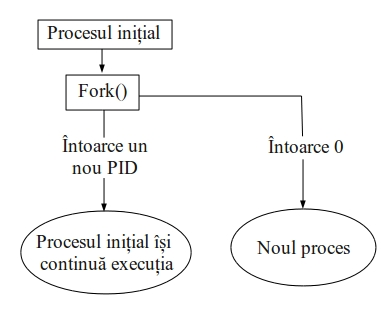
\includegraphics[width=1.8in]{code/fork.jpg}}
			\end{column}
		\end{columns}
		\vspace*{0.2cm}
		\item Windows - organizare neierarhică
		\begin{itemize}
			\item \texttt{CreateProcess} - îmbină cele două operații de pe Linux
		\end{itemize}
		
	\end{itemize}
	
\end{frame}

\begin{frame}{Așteptarea terminării unui proces}
	\begin{itemize}
		\item Linux	
		\begin{itemize}
			\item \texttt{waitpid}, \texttt{wait}
			\begin{itemize}
				\item suspendă execuția procesului apelant până când procesul (procesele) specificat în argumente fie s-au terminat, fie au fost oprite (SIGSTOP)
			\end{itemize}			
			\item \texttt{WIFEXITED}, \texttt{WEXITSTATUS} ...
			\begin{itemize}
				\item obțin modul și codul de ieșire ale procesului, examinând status, întors de waitpid
			\end{itemize}
		\end{itemize}
		\vspace*{0.1cm}
		\item Windows
		\begin{itemize}
			\item \texttt{WaitForSingleObject}, \texttt{WaitForMultipleObjects}
			\begin{itemize}
				\item suspendă execuția procesului curent până când unul sau mai multe alte procese se termină
			\end{itemize}
			\item \texttt{GetExitCodeProcess}
			\begin{itemize}
				\item determină codul de eroare cu care s-a terminat un anumit proces
			\end{itemize}
		\end{itemize}
	\end{itemize}
\end{frame}

\begin{frame}{Terminarea unui proces}
	\begin{itemize}
		\item Linux
		\begin{itemize}
			\item \texttt{exit}
			\begin{itemize}
				\item încheie execuția procesului curent			
				\item toți descriptorii de fișier ai procesului sunt închiși
				\item copiii procesului sunt "înfiați" de \texttt{init}
				\item părintelui procesului îi e trimis un semnal \texttt{SIGCHLD}
				\item va scrie bufferele streamurilor deschise și le va închide
			\end{itemize}		
		\end{itemize}
		\vspace*{0.1cm}
		\item Windows
		\begin{itemize}
			\item \texttt{ExitProcess}
			\begin{itemize}
				\item încheie execuția procesului curent
			\end{itemize}
			\item \texttt{TerminateProcess}			
			\begin{itemize}
				\item încheie execuția altui proces
				\item \textbf{Nu} este recomandată 
			\end{itemize}			
		\end{itemize}
	\end{itemize}
\end{frame}

\begin{frame}{Redirectare}
	\begin{itemize}
		\item Linux	
		\begin{itemize}
			\item \texttt{dup}, \texttt{dup2}
			\begin{itemize}
				\item descriptorii din părinte se moștenesc, implicit, în copil
			\end{itemize}
		\end{itemize}
		\vspace*{0.1cm}
		\item Windows
		\begin{itemize}
			\item descriptorii ce indică fișierele către care se face redirectarea trebuie să poată fi moșteniți în procesul creat
			\begin{itemize}
				\item membrul \texttt{bInheritHandle} al structurii \texttt{SECURITY_ATTRIBUTES} pasate lui \texttt{CreateFile} trebuie să fie TRUE
			\end{itemize}			
		\vspace*{0.1cm}
			\item pentru moștenirea descriptorilor
			\begin{itemize}
				\item parametrul \texttt{bInheritHandle} din \texttt{CreateProcess} trebuie să fie \texttt{TRUE}
			\end{itemize}
		\vspace*{0.1cm}
			\item la crearea procesului, trebuie populată structura \texttt{STARTUPINFO}
			\begin{itemize}
				\item setarea membrilor \texttt{hStdInput}, \texttt{hStdOutput}, \texttt{hStdError} la descriptorii corespunzători
				\item membrul \texttt{dwFlags} trebuie setat la \texttt{STARTF_USESTDHANDLES}
			\end{itemize}
		\end{itemize}
	\end{itemize}
\end{frame}

\begin{frame}{Variabile de mediu}
	\begin{itemize}
		\item Linux
		\begin{itemize}
			\item \texttt{int main(int argc, char **argv, char **environ)} 		
			\begin{itemize}
				\item parametrul \texttt{environ} e un vector de șiruri de caractere de forma VARIABILĂ = VALOARE
			\end{itemize}			
			\item \texttt{getenv}, \texttt{setenv}
			\begin{itemize}
				\item obține/setează valoarea unei variabile de mediu 			
			\end{itemize}
			\item \texttt{unsetenv}
			\begin{itemize}
				\item înlătură o variabilă de mediu 			
			\end{itemize}
		\end{itemize}
		\vspace*{0.1cm}
		\item Windows
			\begin{itemize}
				\item \texttt{GetEnvironmentVariable}, \texttt{SetEnvironmentVariable}			
				\item setarea unei variabile cu valoarea \texttt{NULL} înlătură acea variabilă
			\end{itemize}
	\end{itemize}
\end{frame}

\begin{frame}{Ce este un pipe?}
	\begin{itemize}
		\item mecanisme de comunicare între procese, ce oferă acces de tip FIFO
		\vspace*{0.1cm}
		\item sistemele de operare garantează sincronizarea între operațiile de citire și de scriere la cele două capete
		\vspace*{0.1cm}
		\item două tipuri
		\begin{itemize}
			\item \textbf{anonime}		
			\begin{itemize}
				\item pot fi folosite doar între procese înrudite
				\item există doar în prezența proceselor care dețin descriptori către ele
			\end{itemize}
			\item \textbf{cu nume}
			\begin{itemize}
				\item pot fi folosite între oricare două procese
				\item există fizic - sunt reprezentate de fișiere speciale
			\end{itemize}
		\end{itemize}
	\end{itemize}
\end{frame}

\begin{frame}{Pipe-uri anonime}
	\begin{columns}
		\begin{column} [1]{0.45\textwidth}
			Linux
			\vspace*{0.1cm}
			\begin{itemize}
				\item \texttt{pipe}
				\item \texttt{read}, \texttt{write}
				\item \texttt{close}			
			\end{itemize}
			
		\end{column}
				
		\begin{column} [1]{0.45\textwidth}
			Windows
			\vspace*{0.1cm}
			\begin{itemize}
				\item \texttt{CreatePipe}
				\item \texttt{ReadFile}, \texttt{WriteFile}
				\item \texttt{CloseHandle}
			\end{itemize}
		\end{column}
	\end{columns}

\vspace*{0.5cm}

\textbf{Atenție!} 

\begin{itemize}
	\item \textbf{Linux}: Când se utilizează \texttt{fork}, descriptorii sunt duplicați $=>$ numărul necesar de închideri se vor dubla. Închiderea parțială a descriptorilor conduce la blocaje în \texttt{read}.
	\item \textbf{Windows}: Valorile descriptorilor nu sunt direct vizibile în procesul copil și trebuie făcute cunoscute printr-o metoda alternativă.
\end{itemize}

\end{frame}

\begin{frame}{Pipe-uri cu nume}

	\begin{itemize}
		\item moduri de deschidere
		\begin{itemize}
			\item blocant
			\item neblocant	
		\end{itemize}				
	\end{itemize}

	\begin{itemize}
		\item Linux
		\begin{itemize}
			\item \texttt{mkfifo}
		\end{itemize}
		\vspace*{0.1cm}
		\item Windows
		\begin{itemize}
			\item moduri de comunicare
			\begin{itemize}
				\item flux de octeți
				\item flux de mesaje
			\end{itemize}
			\vspace*{0.4cm}
			%\item arhitectură client-server
		
			\begin{columns}

				\begin{column}  [1]{0.3\textwidth}
					\hspace*{0.5cm} Server
					\item \texttt{CreateNamedPipe}
					\item \texttt{ConnectNamedPipe} 
				\end{column}

				\begin{column}  [1]{0.25\textwidth}
				   \hspace*{0.5cm} Client
					\item \texttt{CreateFile}
					\item \texttt{CallNamedPipe}
				\end{column}
			


			\end{columns}

		\end{itemize}
	\end{itemize}
\end{frame}

%\begin{frame}{Întrebări}
%\begin{itemize}
%\item Care este primul argument (argv[0]) al programului 'fun' dacă se rulează astfel: ./fun so lab 3
%\item Ce va afișa apelul getppid() efectuat de un proces copil al cărui părinte a apelat exit() ?
%\item Câte procese noi se vor crea în urma execuției codului următor: if (fork()) fork();
%\item Ce se întâmplă dacă un program execută următorul cod: execvp(argv[0], \&argv[0])\;
%\end{itemize}
%\end{frame}

\end{document}
